\newcommand{\rtmaude}{Real Time Maude}

\thesischapter{The Application of Real Time Maude to Model and Verify the European Rail Traffic Management System}
The ERTMS system will be central to many train control systems in the future and ensuring that it is safe is of paramount importance. It poses a particular challenge due to the fact that the system is specified at a high level with each individual country having its own particular implementation. One aspect that is particularly problematic and loosely specified is the interface between the existing interlocking and the RBC as both of these systems have a role to play in ensuring safety. In the following chapter we shall look at modelling and then simulating and verifying the ERTMS system whilst capturing the behaviour of this critical interface between the two systems. The simulation of the system provides a validation of our modelling in that it shows the system to be live and that the trains behave as expected. We apply model checking in order to verify that certain safety conditions hold in the model we have specified.

In the following we present the Maude \cite{MC03,Maude} and Real Time Maude \cite{PO02,PO04,RTMaude} tools and describe an approach using these tools to model and verify ERTMS \ref{chapter:ERTMS}.The property we verify is that no two trains on our example railway share the same movement authority which in turn prevents the trains from crashing. We begin by capturing ERTMS as a hybrid automaton which allows us to get a grip of its behaviour. We then prove that a single train automaton always remains within its movement authority. Finally we introduce Maude, Real Time Maude and the Real Time Maude LTL Model Checker which we shall use to model, simulate and formally verify ERTMS. A general introduction to Maude can be found in \cite{MaudeBook}.



\subsection*{Related Work}
The Maude System has been used for a variety of specification and verification tasks. Hardware such has microprocessors has been specified and verified \cite{NH00}. 

On the front of hybrid automata, ERTMS has been verified in the form of Hybrid Automata by translating the automata into a program and then performing model checking using the post condition calculus \cite{DI13}. The Hi-Maude system \cite{MF11} is an extension of Real Time Maude designed specifically modelling interacting hybrid systems and as such it can handle differential equations. It has been used in a case study to model the effects of extreme heat on the human body \cite{MF12}. It is geared towards systems of a highly dynamic nature and may be overkill for a system such as ERTMS with a large discrete component.

There is an example of a distributed sensor network employing the OGDC algorithm that has been modelled and verified using Real Time Maude \cite{PO07}.  The Real Time Maude system can also be used for simulation and analysis of systems as seen in the work on the CASH Scheduling Algorithm \cite{PO06}.

There have been several attempts to model and verify parts of the ERTMS system. The scale of the system and differences in implementations from one country to another both make its formalisation challenging. A subset of the systems requirements specification of ERTMS in UML consisting of high level discrete modes and transitions was captured, formalised and verified using the SMV model checker \cite{MG14}. A variety of properties were checked including safety and liveness which were formalised using modes of the system. One safety condition  "the ETCS on-board never leaves the TRIP mode (TR) before the driver has acknowledged the trip and the train has stopped"\footnote{a train enters the TRIP mode after it has over run its stopping point.}, was formalised as an LTL formula with a boolean variable to represent that the train has stopped, it was then successfully verified using SMV. Our work attempts to capture the more concrete behaviour of the overall system including the physical behaviour of trains such as their speed and that of the highly safety critical interface between ERTMS and the interlocking. 

There has been a large amount of work on the modelling and verification of ETCS using differential dynamic logic \cite{AP08} in the Keymaera tool \cite{AP08b}. The RBC handover where a train moves from the area governed by one RBC into another has been modelled in \cite{YL11}. The properties proven in this study include non-derailment and non collision of trains which follows from correct handover and new movement authority generation. ETCS \cite{AP09} itself has been modelled as a dynamical system with external disturbances and verified for safety in terms of collision avoidence, liveness, controlability and reactivity.

There are also several model checkers specifically for the verification of hybrid systems, including HyTech \cite{AR96} and PHAVer \cite{}, which perform an exhaustive search of the state space to check that a given property holds.

\section{Formalising the European Rail Traffic Management System Using Hybrid Automata}
One formalism which we can use to reason about systems such as ERTMS is hybrid automata \cite{TH96}. We shall give a theoretical overview of Hybrid Automata before formalising ERTMS as three Hybrid automata composed in parallel.
We begin by defining the syntax of a Hybrid automata before defining its semantics in terms of a labelled transition system.
\medskip
\begin{mydef}[Hybrid Automaton: Syntax]
The syntax of a hybrid automaton $H$ comprises of the following:
\begin{description}
\item[Variables] A finite set $X = \{x_1, \ldots x_n \}$ of variables which range over the real numbers. The cardinality of $|X|$ is called the \emph{dimension} of $H$. The variable set has a corresponding dotted variable set $\dot{X} = \{\dot{x}_1, \ldots \dot{x}_n \}$ which represents the continuous changes of variables and a primed variable set $X' = \{x'_1, \ldots , x'_n \}$ that represents  values at the conclusion of a discrete change.

\item[Control graph] A finite directed multigraph $(V,E)$ consisting of a set of vertices which we shall refer to as \emph{control modes} and a set of edges $E$ which we shall refer to as \emph{control switches}.

\item[Initial, invariant and flow conditions] Three functions \emph{init},\emph{inv} and \emph{flow} that label each control mode $v \in V$ with three predicates such that for all $v \in V$, $\freevar{init(v)} \subseteq X$, $\freevar{inv(v)} \subseteq \dot{X}$ and $\freevar{flow(v)} \subseteq X \cup \dot{X}$. 


\item[Jump Conditions] A function \emph{jump} that labels each edge $e \in E$ with a predicate such that $\freevar{jump(e)} \subseteq X \cup X' $.

\item[Events] A finite set $\Sigma$ of \emph{events}, at least one of which is assigned to  each control switch by a labelling function $event: E \to \Sigma$.

\end{description}
Where $\freevar{P}$ is the set of free variables in the predicate $P$.
\end{mydef}
\medskip
A hybrid automaton has discrete states called control modes and transitions between these modes called control switches. These control switches are triggered by either some condition on variables or by some event occurring. These events can either occur in some other automaton or they can be fired by an automaton due to some condition being met. The continuous transitions of the automaton are described by dotted variables and occur continually over time.
\medskip
\begin{myremark}
The dotted variables represent the rate of change of a given variable over time.

$$\dot{y} = \frac{dy}{dt}$$

This notation was introduced by Newton \cite{CF28}.
\end{myremark}
\medskip
The semantics of the hybrid automaton are described using labelled transitions systems. These transition systems allow us to model the behaviour of a system with a possibly infinite number of discrete labelled states. 
\medskip
\begin{mydef}[Labelled Transition System]
We define a \emph{labelled transition system} $LTS = (S,S_0,T,L)$ as follows:
\begin{itemize}

\item $S$ is a possibly infinite set of states

\item $S_0$ is a set of initial states $S_0 \subseteq S$

\item $L$ is a set of \emph{labels}

\item $T$ is a binary relation $\xrightarrow{a}$ over the state space $S$.

\end{itemize}
\end{mydef}
\medskip
When defining the semantics of a hybrid automata we need to be able to speak about parts of the state space.  We define a \emph{region} as being a subset of the state space $R \subseteq S$.  This enables us to define, for example, a continous region for an initial state of a system rather than a discrete state. The semantics of hybrid automata are defined in terms of a timed transition system ...


\medskip
\begin{mydef}[Transition Semantics of Hybrid Automata]
We define the semantics of a hybrid automaton $H$ in terms of a \emph{timed transition system} $LTS^t_H = (S,S_0,L,T)$ as follows:


\begin{itemize}
 
\item The state space $S$ of the timed transition system is defined as, $S, S_0 \subseteq V \times R^n$. A state is in the state space $(v,x) \in S_0$ iff the closed predicate $inv(v)[X := x]$ holds. In addition to the previous condition a state is in the initial state space $(v,x) \in S_0$ iff the closed predicate $init(v)[X := x]]$ holds. We call a subset of the state space $S$ a \emph{H-region}.


\item $L = \Sigma \cup R {\geq 0}$

\item For all events $\sigma \in \Sigma$ such that there exists a control switch $e \in E$, define $(v,x) \xrightarrow{\sigma} (v',x')$ iif the following conditions are satisfied:
\begin{enumerate}
\item the source and target of $e$ are $v$ and $v'$ respectively. 
\item the closed predicate $jump(e)[X, X' := x,x']$ holds.
\item $event(e) = \sigma$.
\end{enumerate}

\item We define a transition $(v,x) \xrightarrow{\delta} (v,x')$ for all non-negative reals $\delta \in R_{\geq 0}$ iff there exists a differentiable function $f: [0, \delta] \to R^n$ such that the following holds:
\begin{enumerate}
\item The functions first derivative is $\dot{f} :(0,\delta) \to R^n$
\item $f(0) = x$
\item $\forall \epsilon \in (0,\delta)$ both of the predicates $inv(v)[X := f(\epsilon)]$ and $flow(v)[X,\dot{X} := f(\epsilon),\dot{f}(\epsilon)]$ hold.
\end{enumerate}
We call the function f the \emph{witness} of the transition $(v,x) \to (v, x')$

\end{itemize}


\end{mydef}
\medskip
The following is a simple example railway we shall use for the purposes of demonstrating our verification approach.  It contains 5 track segments connected to form a pentagon with two trains. This captures most of the behaviours found in a larger more complicated railway as the trains and control systems view any piece of track as a set of track segments joined together to form a route.

\begin{figure} [h!]

\begin{center}
\begin{tikzpicture}[node distance = 3cm]


\node (A) [draw,regular polygon, regular polygon sides=5, minimum size=6 cm,outer sep=0pt] {};
\foreach \n in {1,...,5} {

    \pgfmathtruncatemacro{\value}{(\n - 1) * 50};
    \node at (A.corner \n) [anchor=360/5*(\n-1)+270] {D = \value};
    \node at (A.side \n) [anchor = 360/5 *(\n-1) +270] {$t_{\n}$};
}

\node (B) [draw, rectangle, rotate = 36] at (-1.9,2.6) {Train A};
\node (C) [draw, rectangle, rotate =72] at (3,-1) {Train B};

\end{tikzpicture} 
\end{center}

\label{fig:trackplan2}
 \caption{Pentagon Example}
\end{figure}

\begin{comment}



\def\r{3} 
\def\sone{ \sin 32}
\def\stwo{\sin 72}
\def\cone{\cos 32}
\def\ctwo{\cos 72}
\coordinate(top) at (0,\r);
\coordinate(topleft) at ({ \r * -cos (36)},{ \r * -sin (36)});
\coordinate(topright) at ({ \r * cos (72)}, { \r * -sin (72)});
\coordinate(botleft) at ({ \r * - cos (36)},{ \r * sin (36)});
\coordinate(botright) at ({\r * sin (72)},{\r * cos (72)});

\tikzstyle{box1}=[circle, draw, text width = 2cm, font=\scriptsize]
\tikzstyle{box3}=[rectangle, draw, text width = 2cm, font=\scriptsize]
\tikzstyle{arrow}=[->, thick]
\tikzstyle{biarrow}=[<->,very thick,shorten >=7pt,shorten <=7pt]


\node (A) [font = \scriptsize]  at (topleft)                  {D =150 };

\node (B) [font = \scriptsize]    at (botleft)          {D = 0};

\node (C)[font = \scriptsize] at (top)  { D = 100
						};

\node (D)[font = \scriptsize] at (botright)  { D = 50
						};

\node (E) [font = \scriptsize] at (topright) {D = 200};

\draw [arrow] (D) -- node[right] {$t_1$} (E);
\draw [arrow] (A) -- node[below = 10pt] {$t_4$} (B);
\draw [arrow] (B) --  node[above = 10pt] {$t_2$} (C);
\draw [arrow] (C) -- node [left] {$t_3$} (D);
\end{comment}
We have modelled the ERTMS system controlling the pentagon example (see fig \ref{fig:trackplan2}) using several hybrid automata. In this example the value $D(t)$ represents the distance from the start point at time $t$. 
It contains 2 trains $A$ and $B$ and 5 track circuits $l_0, \ldots , l_4$. The track is uni-directional allowing trains to travel from $0 - 249$. 
\medskip
\begin{myremark}[Train Movement Events]
The following two \emph{train movement events} will be abbreviated in some diagrams:
\begin{align*}
\textbf{train movement events}  \ :=  \ &( \textbf{if} \ D(t) \, mod \, 50 = 0)  \\
  &\textbf{then} \  t_{D(t) \, div \, 50}.t_{(D(t) \, div \, 50) +1} \\
&Train.TrainID.Pos.D(t)
\end{align*} 

\end{myremark}
\medskip
\begin{figure} [h!]

\begin{center}
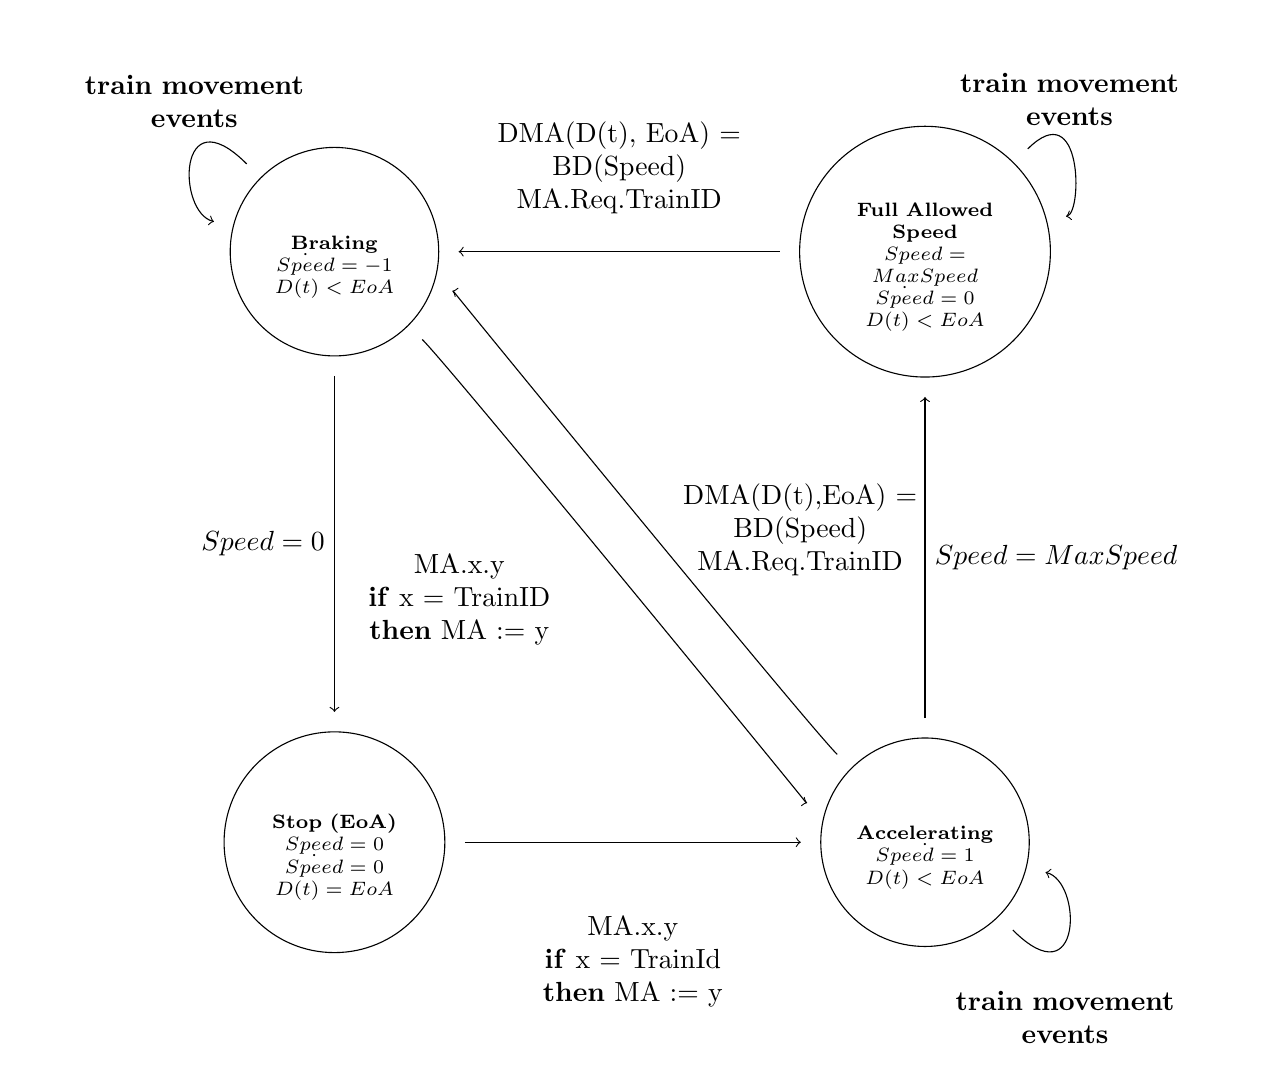
\begin{tikzpicture}[node distance = 2cm]

\tikzstyle{box1}=[circle, draw, text width = 2cm, font=\scriptsize]
\tikzstyle{box3}=[rectangle, draw, text width = 2cm, font=\scriptsize]
\tikzstyle{arrow}=[->,shorten >=7pt,shorten <= 7pt]
\tikzstyle{biarrow}=[<->,very thick,shorten >=7pt,shorten <=7pt]


\node (A) [box1]  at (0,0)                  {\begin{center} \textbf{Stop (EoA)} \\
							$Speed = 0$
                                                        $\dot{Speed} = 0$
							$D(t) = EoA$  \end{center}

                                            };

\node (B) [box1]    at (7.5,0)          {\begin{center} \textbf{Accelerating} \\
       $\dot{Speed = 1}$
       $D(t) < EoA$  \end{center}

};

\node (C)[box1] at (0, 7.5)  { \begin{center} \textbf{Braking}\\
					                   $\dot{Speed} = -1$ 
						           $D(t) < EoA$\end{center}
                                               
						};

\node (D)[box1] at (7.5, 7.5)  { \begin{center} \textbf{Full Allowed Speed }\\
					                   $Speed = MaxSpeed$
                                                            $\dot{Speed} = 0$
							    $D(t) < EoA$
                                                            \end{center}
                                               
						};


\draw [arrow] (B) -- node[right] {$Speed = MaxSpeed$} (D);
\draw [arrow] (A) -- node[below = 10pt, text width = 4cm] {\begin{center}MA.x.y\\ \textbf{if} x = TrainId\\ \textbf{then} MA := y\end{center} } (B);
\draw [arrow] (D) --  node[above = 10pt,text width=4cm] {\begin{center}DMA(D(t), EoA) =\\ BD(Speed)\\MA.Req.TrainID \end{center}} (C);
\draw [arrow] (C) -- node [left] {$Speed = 0$} (A);
\draw [arrow] (B)  .. controls +(-1.5cm,  1.5 cm) and +(1.5cm,  -0.5 cm ) .. node [right,text width=4cm] { \begin{center}DMA(D(t),EoA) =\\
    BD(Speed)\\MA.Req.TrainID \end{center}} (C);
\draw [arrow] (C) .. controls +(1.5cm,  -1.5cm) and +(-1.5cm, 0.5 cm ) ..   node [left,text width = 4cm] {\begin{center}MA.x.y\\ \textbf{if} x = TrainID \\ \textbf{then} MA := y\end{center} } (B);
\draw [arrow] (C) .. controls +(-2cm,  2cm) and +(-2cm, 0.5 cm ) ..   node [above = 10pt, text width = 4cm] {\begin{center}\textbf{train movement events} \end{center}} (C);
\draw [arrow] (D) .. controls +(2cm,  2cm) and +(2cm, 0.5 cm ) ..   node [above = 10pt, text width = 4cm] {\begin{center} \textbf{train movement events} \end{center}} (D);
\draw [arrow] (B) .. controls +(2cm,  -2cm) and +(2cm, -0.5 cm ) ..   node [below = 6pt, text width = 4cm] {\begin{center}\textbf{train movement events} \end{center}} (B);

\end{tikzpicture} 
\end{center}

\label{fig:ContactOrders}
\end{figure}


We start by defining a hybrid automaton for the interlocking consisting of 2 states representing whether a request have been made or not, 5 boolean variables representing whether a track segment is occupied or not and a variable $ReqID$ which stores the last requested track segment. When a request for a track segment is made that track segment is stored and then if the track freedom condition is met then a request is granted, otherwise it is denied. The event $l_x.l_{x+1}$ captures the movement of a train from one track segment to the next in both the interlocking automaton and the train automaton.
\medskip
\begin{mydef}[Interlocking Hybrid Automaton]
We define a hybrid automaton $H_{IL}$ as follows:
\begin{description}
\item[Variables] The state of the interlocking automaton consists of five boolean variables  $\underbrace{l_0, \ldots , l_4}_\text{Occupied/Free}$ and a variable $ReqID$ ranging over $\{0 , \ldots , 4 \}$.

\item[Control Graph] The control graph of the interlocking automaton consists of two control modes $\{Response, Idle \}$ with four control switches connecting them; $Response \to Idle$, $Idle \to Response$, $Response \to Response$, $Idle \to Idle$.

\item[Initial, invariant and flow conditions] \hspace*{0mm}
	\begin{itemize}
	\item $init(Idle) := [l_0 = Free, l_1 = Free, l_2 = Free, l_3 = Free, l_4 = Free]$.

	\end{itemize}

\item[Jump Conditions] \hspace*{0mm}

	\begin{itemize}
	\item $jump(Idle \to Response) :=  Req.z , ReqId' = z$

	
	\item $jump(Response \to Idle) := \mathbf{if} \ (l_{ReqId} = Free \wedge l_{ReqId +1 \, mod \, 5} = Free)$ \\
             \hspace{\fill} $\mathbf{then} \ Grant. ReqId \ \mathbf{else} \ Deny.ReqId$ 

	\item $jump(Idle \to Idle) := l_x. l_{x+1} , [l_x' = Free, l_{x+1}' = Occupied]$

	\item $jump(Response \to Response) := l_x. l_{x+1} , [l_x' = Free, l_{x+1}' = Occupied]$


	\end{itemize}

\item[Events] \hspace*{0mm}
\begin{itemize}
	\item $event (Idle \to Response) := Req.z$
	\item $event(Response \to Idle) :={Grant.z,Deny.z}$
	\item $event(Idle \to Idle) := l_x.l_{x+1}$
	\item $event(Response \to Response) := l_x.l_{x+1}$	
\end{itemize}

\end{description}
\end{mydef} 
\medskip
Before we can describe the behaviour of the train as a hybrid automaton we must first define the equations of motion on which its behaviour is based.
\medskip
\begin{mydef}[Equations of Motion]
The following are equations of motion
\begin{enumerate}
\item $v = u +at$
\item $s = ut + \frac{1}{2}at^2$
\item $s = \frac{1}{2}(u + v)t$
\item $v^2 = u^2 +2as$
\item $s = vt - \frac{1}{2}at^2$
\end{enumerate}
where s = displacement,u = initial velocity, v = final velocity, a = acceleration and t = time.
\end{mydef}
\medskip
Equations number 1 and 4 are the mains one used throughout this formalisation as they allow for the calculation of the breaking distance and speed of a train.
In order to model the behaviour of trains we make use of two functions, one to compute the braking distance at the current speed and the other to compute the distance from the train to the end of the movement authority. When the values computed by these two functions become equal the train should begin to brake in order to stop at the end of the movement authority. The simplest way to model deceleration would be to assume that the trains speed decreases at $-1$ unit of distance per unit of time. Equation of motion (4) is used to caluate the breaking distance with $u = 0$ and $a = 1$ it can be rewritten to allow for the calculation of the breaking distance.

\begin{mydef}[Breaking Distance]
We define the breaking distance for a train in terms of its speed as follows:

$$BD(S) = \frac{S^2}{2} $$


\end{mydef}

\medskip

\begin{mydef}[Distance to MA]

The distance to the movement authority DMA is calulated from the distance and movement authority as followings:
\begin{align*}
DMA(D(t), MA) & = MA \Monus D(t) \quad \mathbf{if} \ DT \leq MA \\
                         & = 50 \Monus D(t) + MA \quad \mathbf{otherwise}
\end{align*}



\end{mydef}

This hybrid automaton has $4$ control modes namely Braking (Auth), Full Allowed Speed, Accelerating and Stopped and has $5$ variables namely $Maxspeed$,$D(t)$ (Position),  $Speed$, $\dot{Speed}$ and $EoA$. We have that $ BD(Speed) \leq DMA(D(t), EoA)$ is an invariant of the stopped mode and $D(t) \leq EoA$ is an invariant of all other control modes.
We define a transition with the event $l_x.l_{x+1}$ which is triggered by the condition $D \,  mod \, 50 = 0$ in the modes $Full Speed$, $Accelerating$ and $Brake$. 
   We compose both the automata for both the interlocking and the hybrid $H_{IL} || H_{T}$. It is possible for a new MA $EoA'$ with $EoA < EoA'$ to be received in the $Braking$ and $Stopped$ states.  This is triggered by the event MA.x.y if $x = TrainID$ then $y$ becomes the new movement authority. The movement event MA.Req.x is used by a train automaton request a movement authority for train x from the RBC automaton.



Secondly we define a hybrid automaton $H_{T}$ which models an individual train. 
\medskip
\begin{mydef}[Train Automaton]

We define a hybrid automaton $H_{T}$ as follows:
\begin{description}
\item[Variables] The state of the interlocking automaton consists of $\underbrace{D(t), EoA}_\text{0, \ldots , 249}$, \newline $\underbrace{Speed, \dot{Speed}, MaxSpeed, TrainID}_{\mathbb{N}}$. The variable D(t) is computed modulo 250 from Speed.

\item[Control Graph] The control graph of the interlocking automaton consists of four control modes $\{Stop (EoA), \, Braking, \, Accelerating, \, Full \, Allowed \, Speed \}$.

\item[Initial, invariant and flow conditions] \hspace*{0mm}
	\begin{itemize}
	\item $init(Stopped) :=   BD(S) \leq DMA(D(t),EoA)  $.

	\item $inv(Full Allowed Speed) :=   \dot{Speed} = 0 \wedge BD(S) \leq DMA(D(t),EoA)$ 

	\item $inv(Accelerating) := BD(S) \leq DMA(D(t),EoA)$

	\item $inv(Braking)  := BD(S) \leq DMA(D(t),EoA)$
	
	\item $inv(Stop (EoA)) := Speed = 0$ 
             
	\item $flow(Accelerating):= \dot{Speed} = 1$ 
	
	\item $flow(Braking) := \dot{Speed} = -1$
 
  
	
	\end{itemize}

\item[Jump Conditions] \hspace*{0mm}

	\begin{itemize}
	\item $jump(Full Allowed Speed \to Full Allowed Speed) := l_{D(t) \, div \, 50}.l_{(D(t) \, div \, 50) +1} \wedge D(t) \, mod \, 50 = 0$
\item $jump(Braking \to Braking) = l_{D(t) \, div \, 500}.l_{(D(t) \, div \, 50) +1} \wedge D(t) \, mod \, 50 = 0$
\item $jump(Accelerating \to Accelerating) = l_{D(t) \, div \, 500}.l_{(D(t) \, div \, 50) +1} \wedge D(t) \, mod \, 50 = 0$

	\item $jump(Stop (EoA) \to Accelerating) := MA.TrainID.y \wedge EoA' = y$ 
	
	\item $jump(Braking \to Accelerating) := MA.TrainID.y \wedge EoA' = y$ 

	\item $jump(Accelerating \to Braking) := DMA(D(t),EoA) = BD(Speed) \wedge MA.Req.TrainID$

	\item $jump(Full Allowed Speed \to Braking) := DMA(D(t),EoA) = BD(Speed) \wedge MA.Req.TrainID$

	\item $jump(Accelerating \to Full Allowed Speed)$ := Speed = MaxSpeed
	
	\item $jump(Braking \to Stop (EoA)) := Speed = 0$

	\end{itemize}

\item[Events] \hspace*{0mm}
\begin{itemize}
	\item $event (Stop (EoA) \to Accelerating) := MA.TrainID.y$
	\item $event (Braking \to Accelerating) := MA.TrainID.y$
	\item $event(Full Allowed Speed \to Full Allowed Speed) := l_{D(t) \, div \, 50}.l_{(D(t) \, div \, 50) +1} \wedge D(t) \, mod \, 50 = 0$
\item $event(Braking \to Braking) = l_{D(t) \, div \, 50}.l_{(D(t) \, div \, 50) +1} \wedge D(t) \, mod \, 50 = 0$
\item $event(Accelerating \to Accelerating) = l_{D(t) \, div \, 50}.l_{(D(t) \, div \, 50) +1} \wedge D(t) \, mod \, 50 = 0$

	\item $event(Accelerating \to Braking) = MA.Req.TrainID$
	\item $event(Full Allowed Speed \to Braking) = MA.Req.TrainID$
\end{itemize}

\end{description}
\end{mydef}



\begin{figure} [h!]

\begin{center}
\begin{tikzpicture}[scale = 0.60]

\tikzstyle{box1}=[circle, draw, text width =3cm]
\tikzstyle{box3}=[rectangle, draw, text width = 2cm, font=\scriptsize]
\tikzstyle{arrow}=[->,shorten >=7pt,shorten <= 7pt]
\tikzstyle{biarrow}=[<->,very thick,shorten >=7pt,shorten <=7pt]



\node (B) [box1]    at (7.5,0)          {\begin{center} \textbf{Idle} \\ \end{center}

};

\node (C)[box1] at (0, 7.5)  { \begin{center} \textbf{Response}\\ \end{center}                                               
						};


\draw [arrow] (B)  .. controls +(-1.5 cm,  2.75 cm) and +(4.5cm,  -2.5cm ) .. node [right, text width=4cm] {Req.z} (C);
\draw [arrow] (C) .. controls +(1cm,  -3cm) and +(-2.75cm, 1 cm ) ..   node [left = 3 cm, below, text width = 6cm] {$Grant.z \  \mathbf{if} \ t_{ReqId} = \ free $\\$ \mathbf{else} \ Deny.z \ Otherwise$} (B);


\end{tikzpicture} 
\end{center}

\label{fig:ILAuton}
\end{figure}


\begin{comment}

\begin{figure} [h!]

\begin{center}
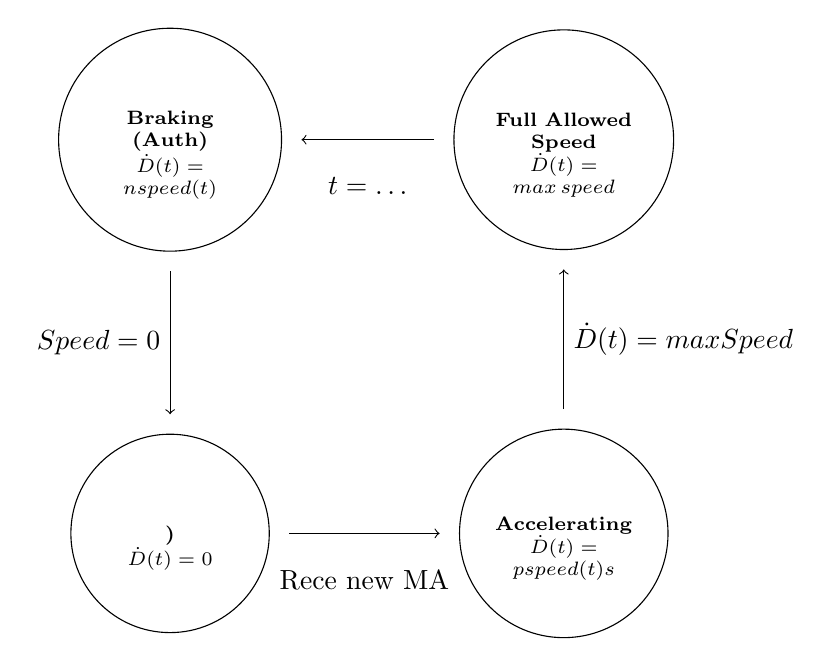
\begin{tikzpicture}[node distance = 3cm]

\tikzstyle{box1}=[circle, draw, text width = 2cm, font=\scriptsize]
\tikzstyle{box3}=[rectangle, draw, text width = 2cm, font=\scriptsize]
\tikzstyle{arrow}=[->,shorten >=7pt,shorten <=7pt]
\tikzstyle{biarrow}=[<->,very thick,shorten >=7pt,shorten <=7pt]


\node (A) [box1]  at (0,0)                  {\begin{center} \textbf{)} \\
							$\dot{D}(t) = 0$  \end{center}

                                            };

\node (B) [box1]    at (5,0)          {\begin{center} \textbf{Accelerating} \\
       $\dot{D}(t) = pspeed(t)s$  \end{center}

};

\node (C)[box1] at (0, 5)  { \begin{center} \textbf{Braking (Auth)}\\
					                   $\dot{D}(t) = nspeed(t)$ \end{center}
                                               
						};

\node (D)[box1] at (5, 5)  { \begin{center} \textbf{Full Allowed Speed }\\
					                   $\dot{D}(t) = max\, speed$ \end{center}
                                               
						};


\draw [arrow] (B) -- node[right] {$\dot{D}(t) = max Speed$} (D);
\draw [arrow] (A) -- node[below = 10pt] {Rece new MA} (B);
\draw [arrow] (D) --  node[below = 10pt] {$t = \ldots$} (C);
\draw [arrow] (C) -- node [left] {$Speed = 0$} (A);


\end{tikzpicture} 
\end{center}

\label{fig:TrainAuton}
\end{figure}
\end{comment}

\medskip
Similarly to the train automaton the RBC automaton also has four control modes namely Granted, Idle, Wait and Ready to Request. Initially the system is in an idle state where the system waits until it receives a movement authority request MA.Req.x. When the train receives such a movement authority request the LastTrain variable is assigned to be x and the system moves to the Ready to Request state.  From this state the train sends a request for the next track segment of the LastTrain.
\medskip

\begin{mydef}[Radio Block Controller Hybrid Automaton]

We define a hybrid automaton $H_{RBC}$ as follows:
\begin{description}
\item[Variables] The state of the radio block controller automaton consists of $\underbrace{MA_1, Pos_1, MA_2, Pos_2}_\text{0, \ldots , 2499}$, \newline $\underbrace{LastTrain}_{\mathbb{N}}$.

\item[Control Graph] The control graph of the radio block controller automaton consists of four control modes $\{Idle, \, Ready \, to \, Request, \, Wait, \, Granted \}$.

\item[Initial, invariant and flow conditions] \hspace*{0mm}
	\begin{itemize}
	\item $init(Idle) :=   \ldots $

	\end{itemize}

\item[Jump Conditions] \hspace*{0mm}

	\begin{itemize}
	\item $jump(Ready to Request \to Ready to Request) := Train.x.Pos.y \wedge MA.x = y$
	\item $jump(Wait \to Wait) := Train.x.Pos.y \wedge MA.x = y$
	\item $jump(Granted \to Granted) := Train.x.Pos.y \wedge MA.x = y$
	\item $jump(Idle \to Idle) := Train.x.Pos.y \wedge MA.x = y$
	\item $jump(Idle \to Ready to Request) := MA.Req.x \wedge LastTrain = x$
	\item $jump(Ready to Request \to Wait) := Req.NextTrack(TrackSeg(Pos.LastTrain))$
	\item $jump(Wait \to Ready to Request) := Deny.LastTrain$
	\item $jump(Wait \to Granted) := Grant.LastTrain$
	\item $jump(Granted \to Idle) := MA.x.EndOf(z)$



	\end{itemize}

\item[Events] \hspace*{0mm}
\begin{itemize}
\item $jump(Ready to Request \to Ready to Request) := Train.x.Pos.y$
	\item $jump(Wait \to Wait) := Train.x.Pos.y$
	\item $jump(Granted \to Granted) := Train.x.Pos.y $
         \item $jump(Idle \to Idle) := Train.x.Pos.y$
	\item $jump(Idle \to Ready to Request) := MA.Req.x $
	\item $jump(Ready to Request \to Wait) := Req.NextTrack(Pos.LastTrain)$
	\item $jump(Wait \to Ready to Request) := Deny.x$
	\item $jump(Wait \to Granted) := Grant.x$
	\item $jump(Granted \to Idle) := MA.LastTrain.EndOf(NextTrack(Pos.LastTrain)))$
\end{itemize}

\end{description}

\end{mydef}



\begin{figure} [h!]

\begin{center}
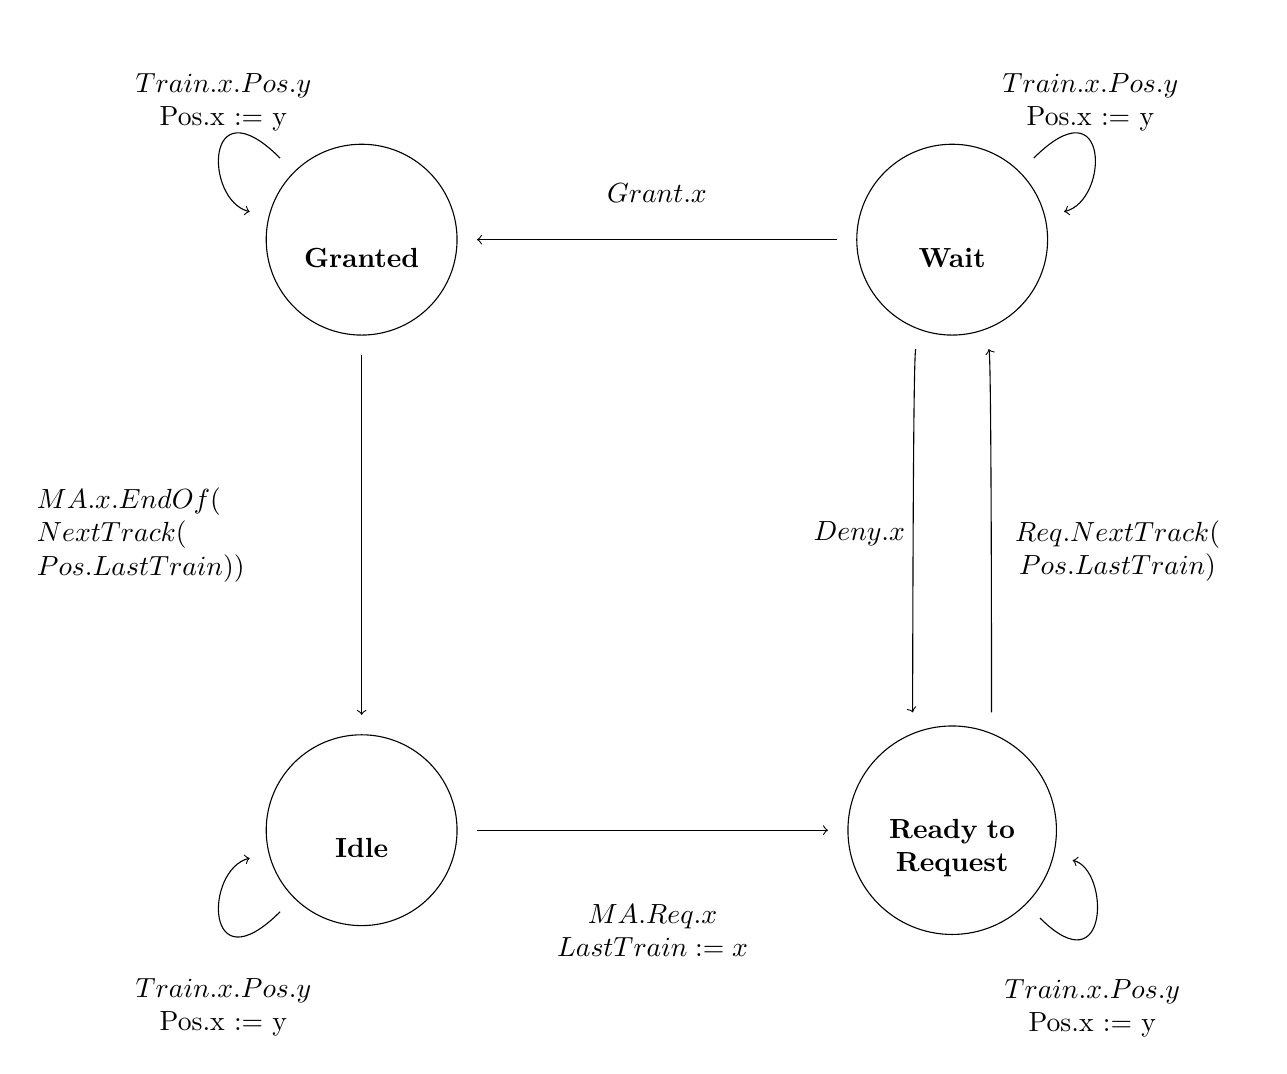
\begin{tikzpicture}[node distance = 1cm]

\tikzstyle{box1}=[circle, draw, text width = 2cm ]
\tikzstyle{box3}=[rectangle, draw, text width = 2cm, font=\scriptsize]
\tikzstyle{arrow}=[->,shorten >=7pt,shorten <= 7pt]
\tikzstyle{biarrow}=[<->,very thick,shorten >=7pt,shorten <=7pt]


\node (A) [box1]  at (0,0)                  {\begin{center} \textbf{Idle} \\
\end{center}};

\node (B) [box1]    at (7.5,0)          {\begin{center} \textbf{Ready to Request} \\
 \end{center}

};

\node (C)[box1] at (0, 7.5)  { \begin{center} \textbf{Granted}\\
					                \end{center}
                                               
						};

\node (D)[box1] at (7.5, 7.5)  { \begin{center} \textbf{Wait}\\
				
                                                            \end{center}
                                               
						};


\draw [arrow] (B)  .. controls +(0.5cm,  1.5 cm) and +(0.5cm,  -1.5 cm ) .. node[right, text width = 3cm] {\begin{center}$Req.NextTrack($ \\ $Pos.LastTrain)$ \end{center}} (D);
\draw [arrow] (D) .. controls +(-0.5cm,  -1.5cm) and +(-0.5cm, 1.5 cm ) ..   node [left] {$Deny.x$} (B);
\draw [arrow] (A) -- node[below = 10pt, text width = 4cm] {\begin{center}$MA.Req.x$ \\ $LastTrain := x$\end{center}} (B);
\draw [arrow] (D) --  node[above = 10pt,text width=4cm] {\begin{center}$Grant.x$\end{center}} (C);
\draw [arrow] (C) -- node [left, text width = 4cm] {$MA.x.EndOf($ \\ $NextTrack($ \\ $Pos.LastTrain))$} (A);

\draw [arrow] (C) .. controls +(-2cm,  2cm) and +(-2cm, 0.5 cm ) ..   node [above = 5pt, text width = 4cm] {\begin{center}$Train.x.Pos.y$\\ Pos.x := y\end{center}} (C);
\draw [arrow] (D) .. controls +(2cm,  2cm) and +(2cm, 0.5 cm ) ..   node [above = 5pt, text width = 4cm] {\begin{center}$Train.x.Pos.y$\\ Pos.x := y\end{center}} (D);
\draw [arrow] (B) .. controls +(2cm,  -2cm) and +(2cm, -0.5 cm ) ..   node [below = 6pt, text width = 4cm] {\begin{center}$Train.x.Pos.y$\\ Pos.x := y\end{center}} (B);
\draw [arrow] (A) .. controls +(-2cm,  -2cm) and +(-2cm, -0.5 cm ) ..   node [below = 6pt, text width = 4cm] {\begin{center}$Train.x.Pos.y$\\ Pos.x := y\end{center}} (A);


\end{tikzpicture} 
\end{center}

\label{fig:RBCAuton}
\end{figure}
\medskip
\begin{mydef}[$q_0$-rooted and initialised trajectories]
Given a labelled transition system $LTS = (S,T,S_0,L)$ and a state $s \in S$. We define a $q_0$-\emph{rooted} \emph{trajectory} as a finite or infinite sequence of pairs $\langle a_i, q_i \rangle_{i \geq 1}$ of labels $a_1 \in L$ and states $q_i \in S$  such that $q_{i-1} \xrightarrow{a_i} q_{i} \in T$ for all $i \geq 1$. If $q_0 \in S_0$ then the sequence of pairs $\langle a_i, q_i \rangle_{I \geq 1}$ is an \emph{initialized trajectory}. 
\end{mydef}
\medskip
\begin{mydef}
We define a live transition system (LTS,A) to consist of a labelled transition system $LTS$ and a set $A$ of infinite initialised trajectories of $LTS$. If for all of the finite initialised trajectories of $LTS$ there exists an infinite trajectory in $A$ such that the finite trajectory is a prefix of the infinite one then we call $A$ \emph{machine-closed}. We define a \emph{trace} $\langle a_i \rangle_{i \geq 1}$ of (LTS,A) to consist of the labels from the either a finite initialised trajectory of $LTS$ or a trajectory in $A$.
\end{mydef}
\medskip

\begin{mydef}[Trace semantics of hybrid automata]
All transitions of a timed transition system $S^t_H$ have an associated \emph{duration} $\delta \in R_{\geq 0}$. Every event $\sigma \in \Sigma$ the transition $q \xrightarrow{\sigma} q'$ has a duration of 0. For all transition $q \xrightarrow{\delta} q'$ where $\delta \in R_{\geq 0}$ the duration is $\delta$.  We define an infinite trajectory $\langle a_i, q_i \rangle_{i \geq 1}$ of a transition system $S^t_H$ to be \emph{divergent} if the sum of the transitions $\Sigma_{i \geq 1} \delta$ is \emph{divergent}.
 \end{mydef}

Safety conditions for the combined system can be separated into discrete and continuous parts.  If we want to specify a safety condition which states that it is not possible for two trains to collide in our current system this could have the following components. 

the continuous part would state that any movement authority issued by the radio block processor would respect the interlockings separation policy. \textbf{(Note: I should up date this part at some point. In the current Maude implementation the interlocking will grant a track segment if it is not occupied)} The discrete part would basically state that there is at least two free track circuits in-between each train.


We will now give a proof by induction that the safety condition "The train will always break on time" holds for a single train automaton.
The base case is that we are in the initial state, the stopped mode, with the invariant $D(t) \leq EoA$. If are in the stopped mode and we receive a movement authority with $EoA > D(t)$ then a jump is performed and move to the accelerating state. Since the transition of time does not cause any flow transitions to occur from the base case we do not need to consider it. In the step case we are in one of the 4 modes (Stopped,Braking,Accelerating,) with the invariant $D(t) \geq BD(EoA,speed)$. In these states jump conditions are considered by performing a case distinction is performed on whether we reach the braking point i.e. $D(t) = BD(EoA, speed)$ or we reach maxspeed the transitions result in states in which the invariants still hold. We also consider flow conditions, if time elapses by some amount $\delta$ we either reach the breaking point $D(t) = BD(EoA,Speed)$ and perform a jump into a state in which the invariant still holds or $D(t) > BD(EoA,speed)$ in which case the invariant $D(t) \leq EoA$ holds. 

Since we have restricted the movement authorities to occur at discrete intervals separated by 50 units of distances we perform induction over the time interval $(0..1)$ in order to prevent multiple mode changes from occurring during the induction step. 
\medskip
\begin{mytheorem}
Given a live transition system $(S^t_{H_{T}},  L^{t}_{H_T}) $

 $$\forall \langle a_i, q_i \rangle_{i \geq 1} \in L^{t}_{H_T}.  \forall (a_n, (v, [D(t), EoA,Speed,\dot{Speed},TrainID])) \in \langle a_i, q_i \rangle_{i \geq 1}$$ $$ \to BD(Speed) \leq DMA(D(t), EoA)$$ 

under the assumption that the max speed of the train and the track segment size (new MA increments) obey the following
                     $$maxspeed + maxspeed^2 < tsegsize$$
\begin{proof}


The proof is performed by fixing a trace $ \langle a_i, q_i \rangle_{i \geq 1}$ and  a label/state pair $(a_n, q_n)$ in the timed trace in which the property holds and then proving that for all possible successor label/state pairs $(a_{n+1},q_{n+1})$. Where  the state $q_n = (v, [D(t), EoA,Speed,\dot{Speed},TrainID])$ and $q_{n+1} = (v', [D(t)', EoA',Speed',\dot{Speed}',TrainID'])$ 

We begin by performing induction on the control mode of the system. 
There are 4 cases for $v$ in which we must argue that the transition $q_n \xrightarrow{a_{n+1}} q_{n+1}$  maintains the property $D(t) \leq EOA$. We then perform induction on the time giving us a further two sub
cases in which the duration of the transition  $\delta = 0$ or $\delta \in \mathbb{R}_{>0}$



\begin{description}
\item[v = Stop] All possible transitions from the stop mode have a duration $\delta = 0$. There is one possible event that $MA.TrainID.y$ which will grant a new movement authority $y$ such that $EoA < y$ and cause a jump to the $Accelerating$ mode with $0 = BD(Speed) \leq  DMA(y,Speed') $


\item[v = Accelerating (Acc)] In the case that the duration of the transition is $\delta = 0$ and only control mode jumps caused by events can occur. The only one of these events that affects the invariant $BD(S) \leq DMA(D(t), EoA)$ is that a new movement authority is received $EoA'$ and since movement authorities are always incremented $DMA(D(t), EoA) < DMA(D(t), EoA')$.
  
In the case that $\delta \in \mathbb{R}_{< 0}$ then a flow transition has occured and we are one of several
possible control modes depending on whether the transition of time triggered a jump or not.  The possibilities are as follows: \\

Acc: The train has accelerated and at not point in time has the distance become equal to the breaking distance therefore the current distance remains below the breaking distance. 


Acc $\to$ Brake: The train has transitioned between three states during the transition of $\delta$  . The transition to the breaking state was causes by the condition $BD(Speed(t_1)) = DMA(D(t_1), EoA)$ at some $t_1$ during the first duration in the Acceleration control mode which remains invariant during the Brake control mode 

Acc $\to$ Brake $\to$ Acc: The train has transitioned between three states during the transition of $\delta$  . The transition to the braking state was caused by the condition $BD(Speed(t_1)) = DMA(D(t_1), EoA)$ being met at some $t_1$ during the first duration in the Acc control mode which remains invariant during the Brake control mode. Then at another time $t_2$ the event MA.TrainID.EoA' occurs meaning a new movement authority has been granted EoA' such that $EoA + tsegsize \leq EoA'$ and the train transitions ot the Accelerating mode once again with the train travelling at $Speed(t_1)$.  At this point the invariant $BD(Speed(t_2)) \leq DMA(D(t_2), EoA')$ holds as we know previously at time $t_1$ that $BD(Speed(t_1)) = DMA(D(t_1), EoA)$ holds and since by the assumption $maxspeed + maxspeed^2 < tsegsize$ it is not possible for the train to travel an entire track segment and therefore $BD(Speed(t_3)) \leq DMA(D(t_3), EoA'')$ holds at all times $t_3$ in the second Acceleration control mode. 


\begin{comment}
 In the $Accelerating$ mode we have $\dot{Speed} = 1$ with $D(t) \leq BD(EoA, Speed) \leq  EoA$. There are two cases either $D(t) = BD(EoA,Speed)$ or $D(t) < BD(EoA,Speed)$.  In the case that $D(t) = BD(EoA,Speed)$  a jump occurs taking the system into the Braking mode
with $D(t_1) = BD(Speed,t_1) < EoA$. In the case that $D(t_1) < BD(Speed,t_1)$ time will progress and at some point in the future $t_2$ the train will with reach the braking point $D(t_2) = BD(Speed',t_2)$ or $Speed' = Max Speed \wedge (D(t_2) < BD(Speed', t_2)$.   In the case that $D(t_2) = BD(Speed', t_2)$ a jump will occur taking the train into the braking mode with $D(t_2) = BD(Speed',t_2) < EoA$. Otherwise $Speed = MaxSpeed$ and a jump is performed to the $Full Allowed Speed$ mode with $D(t_2) < BD(Speed', t_2) < EoA$.
\end{comment}

\item[v = Full Allowed Speed (FAS)]
This is the same as  Accelerating, in the case that the duration of the trainsition is $\delta = 0 $. In the case that $\delta \geq 0$ mode have 4 possible cases 

FAS: The train is travelling at maxspeed and then condition $BD(Speed(t')) = DMA(D(t'), EoA)$ has not been met for all $t'$ in the real interval $\delta$. The invariant therefore continues to hold.

FAS $\to$ Brake: The time interval $\delta$ can be partitioned into two time intervals. The first ending at $t_1$ prior to which the system is in FAS and followed by the Brake mode which ends at $t_2$. The argument from the previous FAS case holds for the first time interval. The end of this time interval marks at point at which the condition $BD(Speed) = DMA(D(t_1), EoA)$ is met and for all subsequent points in time  the braking distance remains equal to the distance to the movement authority.. \\

FAS $\to$ Brake $\to$ Acc: The time interval $\delta$ can be partitioned into 3 time intervals. The first interval in which the system is in FAS ends at $t_1$, period in the Brake mode ends at $t_2$ and finally there is a period in the Acc Mode which ends at $t_3$. The argument for the time interval up to $t_2$ is the same as the argument for the previous FAS $\to$ Brake case. A new movement authority $EoA'$ is granted such that $ DMA(D(t_2), EoA) + 50 =  DMA(D(t_2), EoA')$ causing the jump from Brake to  Acc.  For the whole of the  time period spent in the Acc mode the invariant $D(t_3) < BD(EoA',Speed)$ holds as previously $BD(Speed) = DMA(DT(t_1), EoA)$ and it is impossible for the train to cover a distance of fifty in one time unit.


FAS $\to$ Brake $\to$ Acc $\to$ $FAS$: This follows the same argument as the previous however the time period has been partitioned into four instead of three. The invariant holds in the final FAS state for the same reason as the preceding Acc state as the control mode jump does not have any effect on the distance of the train.

\begin{comment}
wo cases  $D(t) = BD(Speed, t)$ with $t = t_1$ or $t_2$,  $t_1 < t_2$. In the first case a jump occurs instantaneously to the $Braking$ mode with $D(t_1) = BD(Speed, t_1) < EoA$ In the second case time elapses to a point in the future $t_2$ and $D(t)$ increases until $D(t_2) = BD(Speed, t_2)$  then the system will perform a jump to the $Braking$ mode with $D(t_2) = BD(Speed, t_2)  < EoA$. 
\end{comment}

\item[v = Braking]
In the case that $\delta = 0$ there are no 

In the Braking mode with  $\geq \delta \geq 0$ we have $5$ possible cases depending on whether jumps have occurred between the different control modes.

\begin{comment}In the Braking mode there are two cases either $MA.TID.y \wedge Speed > 0$ or $Speed = 0$. Since the train is braking by the definition of $BD$,  $D(t_2) \leq BD(Speed,t_2)$ will continue to hold for any amount of time in this state.  In the case that $MA.TID.y \wedge Speed > 0$ we receive a new movement authority $y$ with $y < EoA$ and a jump is performed to the $Accelerating$ mode with $D(t_2) \leq BD(Speed', t_2) < y$. In the case that $Speed = 0$ a jump occurs to the $Stopped$ state.
\end{comment}

Braking: The first case is that we remain in the braking mode for the duration of the time interval. The invariant $BD(Speed) = DMA(D(t), EoA)$ holds for all times $t'$ in the duration of the interval of the as both the braking distance and distance decrease by the same amount over the time interval.

Braking $\to$ Stopped: The time interval $\delta$ can be partitioned into two separate intervals $t_1,t_2$ corresponding to the duration of time spent in the two control modes.  The argument for the first time interval $t_1$ is the same as that for the previous Braking case. 
The transition from the Braking to Stopped modes is triggered by the speed of the train reaching 0. Up to and including this point in time the invariant $D(t_2) = BD(EoA, Speed)$ holds. For the remainder of the interval $t_2$ the the train is stationary and the invariant continues to hold. 

Braking $\to$ Stopped $\to$ Acc: In this case the time interval $\delta$ can be split up into 3 separate intervals $t_1,t_2$ and $t_3$ corresponding to the 3 control modes. The argument for the first 2 control modes is the same as the argument for the previous case. 
At the end of the interval $t_2$ a new movement authority $EoA'$ has been granted and $D(t_3) < BD(EoA', Speed)$ since the train  has travelled at most one unit of distance during the interval and the movement authority has increased by 50.

Braking $\to$ Acc:  The time interval $\delta$ can be partitioned into 2 separate intervals $t_1$ and $t_2$ corresponding to the two control modes. The argument for the first control mode is same as that as the argument for the first Braking case.  At the end of the interval $t_1$ a new movement authority is received which greatly increases the braking distance far beyond what the train can travel in this possible time interval.

Braking $\to$ Acc $\to$ FAS: The time interval can be partitioned into 3 separate intervals $t_1,t_2$ and $t_3$. The invariant holds in the first two time intervals following the argument from the previous case Breaking $\to$ Acc. At the end of the Acc mode there is a transition to FAS however since there is no possibility of the train reaching the breaking point we know that $D(t_3) < BD(EoA',Speed)$.



\end{description}


\begin{comment}
Initially we are in the stop state and have $D(t) \leq EOA$. There is only one possible transition from this state. we receive a new movement authority with $D(t) < EOA$ and proceed to the accelerating state.
We have two possible cases from the accelerating state. The first case is that the train reaches the braking point and enters the braking state $D(t) = BD(t,speed)$. In this case the trains speed speed will decrease by -1 per unit of time and the train will enter the stop state $EOA$.
The second case is that the train reaches max speed and goes into the maxspeed state. If the train reaches $D(t) = BD(t,speed)$ whilst in the maxspeed state then the train will go into the braking state and the same argument holds from the previous case.
\end{comment}
\end{proof}

\end{mytheorem}


Another interesting property of our model is that alone the model of the interlocking allows for "jumping trains" i.e. it allows for track circuits to become free and occupied in a way that does not model the normal movement of trains.
However when the interlocking automaton is placed in parallel with a train automaton it behaves in a

\begin{mytheorem}

In the composite automaton $H_{IL}|| H_{T} $  the event $t_x.t_{x+1}$ will only occur if  and only if$t_x$ is currently occupied in which case $t_x'$ = free and $t_{x+1}' = occupied$.


\begin{proof}
We have to prove the two directions of the statement. First we prove the $\to$ direction.




Assume a train is in $t_x$ and $((x-1) \ ,mod 5) * 50 \leq D(t) < x *50$.

There are two cases
\begin{enumerate}
\item If the train is in the Stopped state then a $t_{x}.t_{x+1}$ event will never occur as it is not possible in this state.

\item The train is moving i.e. it is in either of the $Accelerating, \, Braking , \,  Full \, Allowed \, Speed$ states. In this case the position of the train will be increasing and eventually it will happen that $D(t) \,  mod \, 50 = 0$. When since $D(t) \, mod \, 50 = 0$  satisfies the jump condition the event
 $t_{x}.t_{x+ 1}$ will occur.  
 

\end{enumerate}
\end{proof}
\end{mytheorem}


\section{Maude}
In the following section we shall describe the term rewriting system Maude. It is a multi-purpose tool containing support for executable-specification, simulation and verification of systems and software. We make use of all 3 of these capabilities and it is this wide range which draws us towards its use. In order to full understand its use in the specification of a real time system we first present a formal and informal definition of a Maude specification followed by an example Maude specification to give insight into theses definitions.



\subsection{Maude Specifications}

A Maude specification consists of \emph{functional modules} declared using \texttt{fmod} and \texttt{endfm} which contain the following:

\medskip
\begin{center}
\begin{tabular}{| c | l |}
\hline
sorts    & \texttt{sort} $s$ or \texttt{sorts}  $s \ s' .$ \\ \hline
subsorts  & \texttt{subsort} $s < s' \ .$ \\ \hline
function symbols  & \texttt{op} $f \ :  \ s_1 \ldots s_n$ \texttt{->} $s \ .$ \\ \hline
variables  & \texttt{vars} $v \ v' : s' .$\\ \hline
uncondition equations  &\texttt{eq} $t = t' .$\\ \hline
condition equations & \texttt{ceq} t = t' \texttt{if} $cond$ \\ \hline
membership axioms & \texttt{mb} $t \ : \ s \ .$ or \texttt{cmb} $t  \ : \ s$ \texttt{if} $cond \ .$  \\ \hline
\end{tabular}
\end{center}

The data types of a Maude specific are defined using sorts with subtypes expressed as subsorts. Terms are constructed using function symbols and variables. These terms are given behaviour using equations and conditional equations.  
%%% Read the Maude papers as this is currently very close to the description of a maude specification found in the RT maude theory paper.
\medskip
\begin{mydef}[Equational Theory]
An equational theory is a 2 tuple $(\Sigma, E)$ where $\Sigma$ is a set of sorts, subsorts and operator declarations  and $E$ is the set of equations modulo $\Sigma$
\end{mydef}

Equational theories  form the signature of a Maude specification and provides one with a means to represent data types using various symbols. If we consider the natural numbers defined symbolically  as an equational theory, the set $\Sigma$ would consist of the sort $Nat$ and the operations $0$, $s$, and $+$, the set $E$ would consist of associativity and commutativity for $+$.

Formally a Maude specification is a \emph{rewrite theory} of the form $\mathfrak{R}=(\Sigma,E,L,R)$, where  $(\Sigma, E)$ is an equational theory, $L$ is a set of labels and $R$ is a set of labelled rewrite rules of the form:

$$ [l] : t \to t' \mathbf{if} \bigwedge^{n}_{i = 1} u_i \to v_i \bigwedge^{m}_{j = 1} w_j = w'_j $$

where $l$ is a label $l \in L$ and $t$, $t'$, $u_i$, $v_i$, $w_j$ and $w'_j$ are implicitly universally quantified variables representing $\Sigma$-terms. Maude theories are \emph{order-sorted} allowing for the specification of subsorts which is achieved by including into the specification a partial order relation over sorts. Given two sorts $s$ and $s'$ this partial order relation $s \leq s'$ is interpreted as subset inclusion $A_s \subseteq A_{s'}$ in a model $A$.

The behaviour the operations defined in an equational theory are defined in a rewrite theory using the labelled rewrite rules. In the case of the natural numbers it is then possible to provide an definition for $+$ recursively. The base case is where 0 is one of the operands in which case we return the other $0 + N \to N$. The successor case is that we have some non-zero operand represented as a successor to some variable $s(M)$ in which case we apply the successor function to the recursive call of addition with M and the other operand $s(M) + N \to s(M + N)$. 
 

\subsubsection{Example Maude Specification}
We shall now give a small example specification in the form of the natural numbers in Maude in order to get a feel for the structure of such a specification. We see that the module BASIC-NAT on the first line of the example (CL \ref{code:natnum}). Followed by a sort Nat which forms the type with which we will be working. Next several operations are declared with which we define the natural numbers symbolically. Firstly, we see a 0 operator which forms our basic constructor which is followed by another operation s which allows us to construct successive natural numbers. The infix addition operation $+$ defined using variable place holders  $\_$. The behaviour of the addition operation is defined inductively using two variables N and M and two equations for the base and successor cases.

\begin{lstlisting}[caption = The natural numbers in Maude, label = code:natnum]
fmod BASIC-NAT is
        sort Nat .

        op 0 : -> Nat .
        op s : Nat -> Nat .
        op _+_ : Nat Nat -> Nat .

        vars N M : Nat .

        eq 0 + N = N .
        eq s(M) + N = s(M + N) .
endfm
\end{lstlisting}



\section{Real Time Maude}
One extension of Maude that has been used to model and verify hybrid systems is Real Time Maude. This contains specific support enabling the modelling and verification of real-timed and discrete timed systems. It is stated by its developers that Real Time Maude is not first and foremost a verification tool. This is due to some inherent limitations in LTL-model checking that hinder the verification of infinite state systems. We have, as in the sensor network example, only model checked a portion of the state space of our example using this tool. This is however enough to have confidence in the correctness of the system with respect to a given safety condition.


\subsection{Real Time Maude Specifications}
A Real Timed Maude specification consists of \emph{timed modules} that start with \texttt{tmod} and end with \texttt{endtm}. Formally a Real Time Maude specification is a real-time rewrite theory which can be thought of as a rewrite theory with an interpretation for the abstract time domain together with rewrite rules for terms of type \texttt{System} that have a time duration \cite{PO02}. These rewrite rules can be separated into two categories, the \emph{tick} rules have a non-zero time elapse and the \emph{instantaneous} rules have a time elapse of zero.

The interpretation of the abstract time domain is mapped to a concrete specification of time during the specification process. Real time Maude comes with two of these specifications as standard the most simple  is discrete time based on the natural numbers and the more complicated of the two is dense time based on the rational numbers. We shall use discrete time during the specification as it allows for the best results during the verification process. 

\medskip

\begin{mydef}[Equational Theory Morphism]
 We define an \emph{equational theory morphism} $H: (\Sigma,E) \to (\Sigma', E')$ to consist of the following
\begin{itemize}
\item a monotone map $H:sorts(\Sigma) \to sorts(\Sigma')$ which maps  sorts in $\Sigma$  to sorts in $\Sigma'$

\item a mapping which maps every function symbol $f : s_1 \ldots s_n \to s$ in $\Sigma$ to some term $H(f_{s_1 \ldots s_n, s})$ from $\Sigma'$ of sort $H(s)$ such that the following conditions are satisfied:
\begin{enumerate}

\item  $\var{H(f_{s_1 \ldots s_n, s})} \subseteq {x_1:H(s_1), \ldots, x_n:H(s_n)}$

\item if the operator $f: s_1 \ldots s_n \to s$ can be subsort overloaded $f: s'_1 \ldots s'_n \to s'$ such that $s_i \leq s'_i, s\leq s'$ then it is possible to substitute each variable $x_i:H(s'_i)$ by the corresponding variable $x_i:H(s_i)$ in the term $H(f_{s'_1 \ldots s'_n, s})$ and obtain $H(f_{s_1 \ldots s_n, s})$.

\item For every axiom: $$(\forall y_1:s_1, \ldots y_k : s_k) u = v \ \textbf{if} \ C$$ in E the homomorphic extension of $H^*$ to terms and equations in the condition $C$ causes the following to hold:
   $$E' \models (\forall y_1 : H(s_1), \ldots, y_k : H(s_k)) H^*(u) = H^*(v) \ \textbf{if} \ H^*(C)$$

\end{enumerate}

\end{itemize}

\end{mydef}
\medskip

A real time rewrite theory is a rewrite theory combined with some concrete implementation of time based on the abstract time domain defined in the time theory. The equational theory morphisms are used to map objects and morphisms in the abstract time domain to the concrete implementation.

\medskip
\begin{mydef}[Real-Time Rewrite Theory]
We define a \emph{real-time rewrite theory} $\mathfrak{R}_{\phi,\tau}$ to be a tuple $(\mathfrak{R}, \phi,\tau)$ containing a rewrite theory $\mathfrak{R} = (\Sigma, E,L,R) $ where:

\begin{itemize}
\item $\phi$ is an equational theory morphism $\phi : \mathit{Time} \to (\Sigma, E)$ that maps objects in the theory \textit{Time} to objects in the equational theory $(\Sigma , E)$.

\item The time domain is functional i.e. if a term $r$ of sort $\phi(Time)$  has a rewrite proof $\alpha: r \to r'$ then $r = r'$ and the identity proof of $r$ is equivalent to $\alpha$.

\item There is a designated sort typically called \textit{State} and a sort \textit{System}, contained within $(\Sigma, E)$, which has no supersorts or subsorts and only one operator that does not satisfy any non trivial equations:

$$\{\_\}: State \to System$$

Further to this condition, it is all required that the sort \textit{System} does not appear in $s_1, \ldots s_n$ the domain  of  any operator $f: s_1, \ldots s_n$.

\item For each rewrite rule with $u$ and $u'$ of sort \textit{System} in $\mathfrak{R}$ of the following form\footnote{All other rules which are not of this form are called \emph{local} rules and have an instantaneous zero time elapse. These do not act on the system as a whole but rather on one or more of its components.}:

there is an assigned term $\tau_l(x_1 \ldots x_n)$ of sort $\phi(Time)$ within $\tau$.

\end{itemize}
\end{mydef}
 
\subsubsection*{Example Real Time Maude Specification}
The following a very simple model of a train Real Time Maude that moves one unit of distance in one time unit along a circular track of length 500. It defines a sort \texttt{TrainState} and a single state \texttt{move}. We have a constructor train of type \texttt{System} which consists of a train state and a natural number.  

\begin{lstlisting}
(tmod DISCRETE-SINGLE-TRAIN is protecting NAT-TIME-DOMAIN .
  sort TrainState .
  ops  move :  -> TrainState [ctor] .
  op train : TrainState Nat -> System [ctor] .
 
  vars N : Time .
  crl [travel] : {train(move,N)} => {train(move,N + 1)} 
                                      in time 1 if N < 500 .
  rl [reset] : {train(move,500)} => {train(move,0)} . 
         
endtm)
\end{lstlisting}
There is a condition rewrite rule called travel which enables the train to move as long as its current distance is less than 500. There is a reset rule that instantaneously resets the trains distance back to zero when it reaches 500.


\subsubsection*{Executing a Real Time Maude Specification}
Real Time Maude allows one to execute or simulate a real time system by applying rewriting rules to a term of type \texttt{System}.
The command \texttt{(trew \{System\} in time <= t)} will attempt to rewrite the system to a state $t$ time units in the future. This is not always possible though as the system may deadlock. The following command attempts to rewrite a train, which initially has distance $0$, to its state in 100 units of time in the future: 
\begin{center}
\texttt{(trew {train(move,0)} in time $\leq$ 100 .)}
\end{center}

The result from this timed rewrite is as follows:
\begin{lstlisting}
rewrites: 4027 in 4ms cpu (3ms real) (1006750 rewrites/second)

Timed rewrite  {train(move,0)} in DISCRETE-SINGLE-TRAIN 
with mode deterministic time increase in time <= 100

Result ClockedSystem :
  {train(move,100)} in time 100
\end{lstlisting}

The ability to perform such simulations is useful as it allows for the liveness of a system to be checked. It also provides another way of validating the correctness of a model by perform many of these executions and checking the behaviour of the system over time.

\subsection{Object Orientated Specification in Real Time Maude}
Real Time Maude is based on Full Maude which contains message and object constructs for object orientated specification. Using these constructs its possible to model ERTMS as several synchronously communicating processes. A Real Time Maude specification consists of  \emph{timed object orientated modules} which start with \texttt{tomod} and end with \texttt{endtom}.
\medskip
We can define the following:
\begin{align*}
\textbf{classes}: & \texttt{ class C | a1 : ⟨Sort-1⟩, ... , an : ⟨Sort-n⟩ . } \\
\textbf{objects}: & \texttt{ < O : C | a1 : v1, ... , an : vn >  . } 
\end{align*}
where $C$ is the class identifier $O$ is the object name  $a_1 \ldots a_n$ are attribute names and $v_1 \ldots v_n$ are values. \\
\medskip
To model communicating processes Real Time Maude uses a messages construct.
\begin{center}
\verb|msgs M1 ... Mn : Sort-1 ... Sort-n -> Msg . | 
\end{center}


\subsubsection*{Configurations in Real Time Maude}
Objects and messages in a specification are given a sort of \texttt{Configuration} which is a subsort of type \texttt{System}. The composition operation for these configuration allows for a combination of objects and messages to form new configurations. This composition operation is also commutative meaning the order of messages and objects in any configuration is ignored. This allows for more generalised writing rules in an object orientated specification that speak about specific objects and messages that are part of some bigger configuration that does not affect the firing of the rule.

\begin{lstlisting}[caption = The Maude Configuration module]
mod CONFIGURATION is  
    *** basic object system sorts  
    sorts Object Msg Configuration .  
 
    *** construction of configurations  
    subsort Object Msg < Configuration .  
    op none : -> Configuration [ctor] .  
    op __ : Configuration Configuration -> Configuration  
         [ctor config assoc comm id: none] .
\end{lstlisting}



\subsubsection*{Example Object Orientated Specification}
The following is an example consisting of two classes of object which serves to demonstrate some of the advantages of object orientated specification as well as some of the pit falls. Firstly there is the class defining D objects which count modulo 500 and transmit a message containing the current count. Secondly there is class defining a object B that reads messages from a D object. 

\begin{lstlisting}[caption = Example object orientated specification, label = code:rtmaudeexample]
(tomod EXAMPLE1 is protecting NAT-TIME-DOMAIN .
  msgs msgD  : Nat -> Msg .  
  class  D | d : Nat .
  class  B | b : Nat .
  vars N: Nat .
  var O : Oid .
  var REST : Configuration .
 
  rl [makeD] : {< O : D | d : N > REST} => 
  {msgD(N + 1 rem 500)  
  < O : D | d : (N + 1) rem 500 > REST} in time 1 . 

  rl [readB] : {msgD(N) < O : B | > REST} => 
  {< O : B | b : N > REST}  . 
endtom)
\end{lstlisting}

We can execute the specification as follows:
\begin{center}
\texttt{(trew {< myD : D | d : 0 > < myB : B | b : 0 >} in time <= 2 .)}
\end{center}

Resulting in the following output:
\begin{lstlisting}
rewrites: 6246 in 7ms cpu (7ms real) 
(805000 rewrites/second)

Timed rewrite  {< myD : D | d : 0 > < myB : B | b : 0 >} 
in EXAMPLE1 with mode deterministic time 
increase in time <= 2

Result ClockedSystem :
  {< myB : B | b : 2 > < myD : D | d : 2 >} in time 2
\end{lstlisting}

The Maude system rewrites the initial state of the system into the resulting state however that does not mean that this is the only reachable state. This set has some non-determinism in that we do not force the messages to be read immediately and the rewriting equations could be applied in any order. There is a reachable state in time 2 in which both of the messages have not been read meaning that either of them could be read in any order resulting in  . 
The following are some states reachable in time 2.

\begin{lstlisting}[caption = Some of the states reachable by rewriting EXAMPLE1 in two time steps, label = code:reachst ]
{< myB : B | b : 1 > < myD : D | d : 2 >}
{< myB : B | b : 2 > < myD : D | d : 2 >}
{msgD(1)< myB : B | b : 2 > < myD : D | d : 2 >}
{msgD(1)msgD(2)< myB : B | b : 0 > < myD : D | d : 2 >}
{msgD(2)< myB : B | b : 1 > < myD : D | d : 2 >}
\end{lstlisting}

\emph{Non-determinism} should be avoided unless it is really is a property you want in a model. One way to remove some of these reachable states is to make the variable \texttt{REST} of sort \texttt{ObjectConfiguration}. This forces objects of the B class to read messages after each incrementation of time. If we make this modification to the specification then the following states, from code listing \ref{code:reachst}, are reachable in time 2.
\begin{lstlisting}
{< myB : B | b : 2 > < myD : D | d : 2 >}
{msgD(2)< myB : B | b : 1 > < myD : D | d : 2 >}
(msgD(1)< myB : B | b : 0 > < myD : D | d : 1 >}
(< myB : B | b : 1 > < myD : D | d : 1 >}
\end{lstlisting}


\section{Modelling the European Rail Traffic Management System}
In the following we shall give an overview of the specifications used to model the ERTMS system. We have used the Real Time Maude system in an object orientated fashion following the hybrid automata described in \ref{} to define one class for each of the 3 hybrid automata.
\subsubsection*{Modelling the Transition of Time}
In our previous Real Time Maude specifications we have had a rewrite rules that work on a specific object or state and increment time for the whole system. This presents a problem as we could have two objects that can both increment the time of the global system independently. We need a way of incrementing the time of the whole global system and then distributing this increment of time amongst the objects of the system. To solve this problem we define operator $\delta$ which describes how distributed system evolves with time.

\begin{lstlisting}[caption = The delta time transition operation, label = code:delta]
op delta : Configuration -> Configuration [frozen] . 

var OCREST : ObjectConfiguration .

rl [timetrans] : {OCREST} => {delta(OCREST)} in time 1 .
rl [delta1] : delta(CON1 CON2) => delta(CON1)delta(CON2) .
\end{lstlisting}

The operation delta is frozen meaning that the configuration contained within will not be evaluated by the Maude until the delta operation has been evaluated. We only allow for time to be incremented on a global system containing an object configuration which cannot by definition contain any messages. This forces all messages sent in one time interval to be read during that interval. The delta1 rule distributes the deltas over the constituent objects of a configuration until there are many deltas applied to configurations containing singleton objects. Each of these singleton objects has its own seperately defined behaviour for the delta operation that captures that transition of time for that object. This was inspired by  \cite{} where a delta operation is used to distribute time over a distributed sensor network. 

\subsubsection*{Modelling Trains}
We shall now describe the specification of trains. We define the Train class to have a state which like our hybrid automata can be in one of 4 possibilities, constant speed, accelerating, stopped and breaking. As well as the state it also has 6 fields of sort Nat representing the distance, speed, acceleration, movement authority,  current track segment and max speed.

\begin{lstlisting}
sort TrainState .
ops  cons acc stop break :  -> TrainState [ctor] .

class Train | state : TrainState, dist : Nat, 
      speed : Nat, ac : Nat, ma : Nat, 
      tseg : Nat, maxspeed : Nat .
\end{lstlisting}

We capture the behaviour of trains using a number of instantaneous and tick rewriting rules. The instantaneous rules are used to capture a change of state within a train. For example if the a train is in the cons state distance to the movement authority becomes less than the distance needed to break to zero in the next moment of time one of these rules will fire and cause a state transition. 

We compute the breaking distance as follows: 
\begin{center}\texttt{eq bd(S) = (S * S) div 2 .}\end{center}


The division operation is based on repeated subtraction and finally taking the floor or the resulting number. When we divide a number by two in the breaking function we add 1 to change this to the ceiling of the resulting number. This prevents a situation where we have a distance of 1 from our moment authority but the breaking distance is zero.
The distance to the movement authority to the train is computed by:
\begin{center}
\texttt{} \\
\texttt{}
\end{center}

When modelling the trains we perform the jumps from accelerating and full allowed speed to breaking if the breaking distance becomes less than the distance to movement authority in the next moment in time.


\subsubsection*{Sets and Maps in Maude}
In order to have more general data types Maude allows for parametrised functional modules with the  syntax \texttt{fmod M{$X_1$ :: $T_1$ , $\ldots$ , $X_n$ :: $T_n$} is $\ldots$ endfm} where $n \geq 1$, $X_1$ is the \emph{parameter name} and $T_1$ is the \emph{theory name}.

In the formalisation of the RBC we make use of the Map data type to store the position and movement authority of a given train and we use a Set to store trains that have made requests in the current time interval. 

\begin{lstlisting}[caption = The specification of the Set data type in Maude]
fmod SET{X :: TRIV} is 
 protecting EXT-BOOL .
 protecting NAT .
 sorts NeSet{X} Set{X} .
 subsort X$Elt < NeSet{X} < Set{X} .

 op empty : -> Set{X} [ctor] .
 op _,_ : Set{X} Set{X} -> Set{X} .
 
 op insert : X$Elt Set{X} -> Set{X}
 eq insert(E, S) = E, S

 op _in :: X$Elt Set{X} -> Bool .
 eq E in (E, S) = true.
 eq E in S = false [owise] .

\end{lstlisting}

The indivudal elements the set are themselves are a subsort of set, allowing for sets to be constructed using the union operater \texttt{\_,\_} and singleton sets. The in operation computes set membership and is based on the \texttt{otherwise}  meaning that false case will only be applied once the search for true case has been exhausted.

\begin{lstlisting}[caption = The specification of the Map data type in Maude]
fmod MAP{X :: TRIV, Y ::  TRIV} is
 protecting BOOL .
 sorts Entry{X,Y} Map{X,Y} .
 subsort Entry{X,Y} < Map{X,Y} .

 op _|->_ : X$Elt Y$Elt -> Entry{X,Y} [ctor] .
 op empty : -> Map{X,Y} [ctor] .
 op _,_ : Map{X,Y} Map{X,Y} -> Map{X,Y} 
     [ctor assoc comm id: empty prec 121 format (d r os d)] .
 op undefined : -> [Y$Elt] [ctor] .

 var D: X$Elt .
 vars R R' : Y$Elt .
 var M : Map{X,Y} .

op insert : X$Elt Y$Elt Map{X,Y} -> Map{X,Y} .
eq insert(D, R,(M, D |-> R'))
   = if $hasMapping(M, D)
    then insert(D, R, M)
    else (M, D |-> R)
    fi .
eq insert(D, R, M) = (M, D |-> R) [owise] .

op $hasMapping : Map{X, Y} X$Elt -> Bool .
eq $hasMapping((M, D |-> R), D) = true .
eq $hasMapping(M, D) = false [owise] .

op _[_] : Map{X,Y} X$Elt -> [Y$Ellt] [prec 23] .
eq (M, D |-> R) [D]
   = if  $hasMapping(M, D) then undefined else R fi .
eq M[D] = undefined [owise] .
\end{lstlisting}
A Map from type $X$ to type $Y$ consists of entries constructed using the $\_|->\_$ operation on an element of type $X$ and an element of type $Y$. These entries are composed together using the commutative and associative opertation $\_,\_$ to form a Map.  

When we use a parametrised data type in a specification it is possible to assign a new sort to the particular parametrised instance of the map or set that we are using.
\begin{center}
\texttt{protecting MAP\{Oid,Nat\}  * (sort Map\{Oid,Nat\} to MapON,
                               sort Entry\{Oid,Nat\} to EntryON) .}
\end{center}




\subsubsection*{Modelling the Radio Block Processor}
The RBC is slightly differently from the hybrid automaton described previously. Instead of having four states the RBC has three states with the behaviour of the granted state being combined into the behaviour of a transition which causes the RBC to leave the wait state. The when the RBC receives a track segment grant fromt the interlocking it immediately grants the movement authority before going back to the idle state.
 
\begin{lstlisting}[caption = The RBC state and class definition in Maude]
sort RBCState .
ops rbcidle ready wait :  -> RBCState [ctor] .
class RBC | state : RBCState, lasttrain : Oid, ma : MapON, 
      pos : MapON , curreq : SetO .
\end{lstlisting}

We use maps to store the current movement authorities and positions of the various trains. In order to prevent an infinite amount of requests being made to an interlocking we limit the rbc to make one request on behalf of each train to the interlocking.  To do this we use  \texttt{curreq}, a set of oids, to store which trains have had a request made for them at a given moment of time.

An example RBC transition is as follows:
\begin{lstlisting}[caption = The state transition for the granting of a movement authority]
rl [rbcgrant] : {grant(N) < O : RBC | state : wait, 
   lasttrain : T1, ma : MAP1  > REST} => 
   { < O : RBC | state : rbcidle, 
       ma : insert(T1,endoftrack(N),MAP1) > 
     grantma(T1, endoftrack(N)) REST} .
\end{lstlisting}

This transition captures two of the state transitions in our RBC automaton. Once the interlocking has granted a request to the RBC for track segment $N$ the RBC immediately proceeds to simultaneously update the movement authority mapping entry for that train and issues a \texttt{grantma} message to that train with a new movement authority for the end of track segment $N$.

\subsubsection*{Modelling the Interlocking}
An interlocking has two states, either it is idle or it has received a request for a movement authority and must respond. We define an Interlockings state and class in Real Time Maude as follows:

\begin{lstlisting}[caption = The interlocking class and states in Maude]
sort InterState .
ops idle res :  -> InterState [ctor] .
class Inter | state : InterState, reqid : Nat, 
      t0 : Bool, t1 : Bool, t2 : Bool, 
      t3 : Bool, t4 : Bool .
\end{lstlisting}

The sort \texttt{InterState} models the state of the interlocking along with two constant operations idle and res which represent the two states. The interlocking class consists of a interlocking state, a request id which stores the current track segment requestions and 5 Booleans which indicate whether or not a track segment is occupied. We define an Interlocking class in Real Time Maude as follows:


All of the rewrite rules on Interlocking objects are instantaneous and do not effect the transition of time.  We can split these rules into two types. Firstly there are interlocking rules that deal with the transition of a train from one track segment to another. Secondly there are several rewriting rules that deal with granting or denying a received request. There is currently a rule for both denying and granting a request for each track segment depending on the value of the boolean variable.

\begin{lstlisting}[caption = The interlocking transition which grants a track segment request]
rl [resreq1g] : {< O : Inter | state : res, t
   1 : false,  reqid : 1 > REST} => 
   {< O : Inter | state : idle > grant(1) REST} .
\end{lstlisting}

\subsection{Simulating the European Rail Traffic Management System Using Real Time Maude}
We will now see how this executable specification can be used to simulate and obtain a better understanding of the modelled system. For this purpose we have written a small Haskell program that takes the output from multiple timed rewrites and plots them as a graph.

In the following we use an example initial state containing two trains one of which is slower (train1) than the other (train2), an interlocking and a radio block processor. The faster train will eventually catch up with the slow train and it waits for that train to clear all successive track segments before proceeding. The trains start at positions on opposing sides of the track with train1 starting at 0 and train2 starting at 150. The RBC and the interlocking are both initialised with the trains in these positions. In Maude this initial state is modelled as follows. Firstly, we define the initial states of the component objects individually:

\begin{lstlisting}[caption = The initial interlocking state in Maude]
 eq initialintstate2 = < inter1 : Inter | state : idle, 
                         reqid : 0, t0 : true, 
                         t1 : false, t2 : false, 
                         t3 : true, t4 : false > .
\end{lstlisting}

The  interlocking is initially idle, the request variable is set to zero, the track segments containing trains are set to true and the remaining track segments are set to false.

\begin{lstlisting}[caption = The initial RBC state in Maude]
 eq initialrbcstate2 = < rbc1 : RBC | state : rbcidle, 
                         lasttrain : train1,  
                         ma : (train1 |-> 49, train2 |-> 199), 
                         pos : (train1 |-> 0, train2 |-> 150), 
                         curreq : empty > .
\end{lstlisting}

Like the interlocking, the RBC is also initially idle. Since the lasttrain variable has not effect in this state and will be set in any successive control flow we simply set it to be train1. The movement authorites  and positions of the trains are set within the ma and pos mapping respectively and the current request is empty.  

\begin{lstlisting}[caption = The intital state of train2 in Maude]
 eq initialtrainstate1 = < train1 : Train | state : acc,  dist : 0, 
                           speed : 0, ac : 1, ma : 49, 
                           tseg : 0, maxspeed : 4 > .
\end{lstlisting}
We set the train1 to be accellerating initally with a distance and speed of zero its movement authority is fourty nine , it is in the zero track segment and has a maxspeed of four. 

\begin{lstlisting}[caption = The intial state of train2 in Maude]
eq initialtrainstate2  = < train2 : Train | state : acc, dist : 150, 
                           speed : 0, ac : 1, ma : 199,
                           tseg : 3, maxspeed : 7 > .
\end{lstlisting}
Like train1, train2 is also accellerating initially and has a speed of zero.  Unlike train1 it has a distance of one hundred and fifty, a movement authority of one hundred and ninty nine, it is in the fourth track segment number three and has a maxspeed of four. Both trains have an accelleration of one. 

Using these initial states for the individual objects we can form the initial state for our pentagon example using the following command:
\begin{lstlisting}
 eq initialstate2 = {initialtrainstate1 initialtrainstate2 
                         initialintstate2  initialrbcstate2} . 
\end{lstlisting}
The operation initial state 2 is of type System and contains a Configuration consisting of the initial states of train1, train2, the rbc and the interlocking. This initial state forms a model of ERTMS which we can simulate using Real Time Maude to rewrite it to a state after a set number of time steps. The model of ERTMS is executed using the following command:
\begin{center}
\texttt{(trew initialstate2 in time $\leq$ 50 .)}
\end{center}

In the resulting output at time 50 both of the trains have moved a considerable distance and have requested and received new movement authorities.
 
\begin{lstlisting}[caption = The result of rewriting initialstate2 for 50 time steps]
Result ClockedSystem :
  {< inter1 : Inter | reqid : 3,state : idle,
     t0 : false,t1 : false,t2 : true,
     t3 : true,t4 : false > 
   < rbc1 : RBC | curreq : train2,lasttrain : train2,
     ma : (train1 |-> 199, train2 |-> 149),
     pos : (train1 |-> 180, train2 |-> 122),
     state : rbcidle > 
   < train1 : Train | ac : 1,dist : 184,ma : 199,maxspeed : 4,
    speed : 4,state : cons,tseg : 3 > 
   < train2 : Train | ac : 1,dist : 128,ma :
    149,maxspeed : 7,speed : 5,state : break,tseg : 2 >} in time 50
\end{lstlisting}

\begin{figure}
\begin{center}
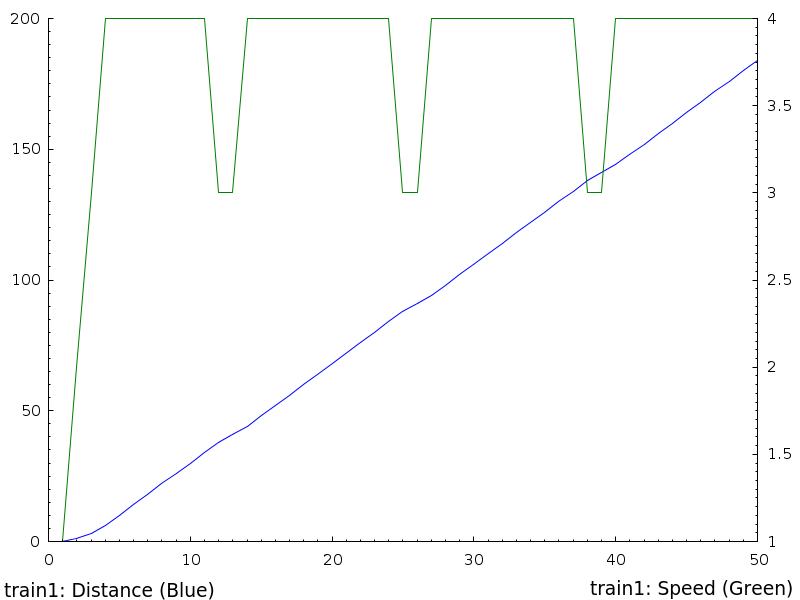
\includegraphics[scale=0.5]{t1graph.png}
\end{center}
\caption{A graph comparing the distance and speed of train1}
\end{figure}

\begin{figure}
\begin{center}
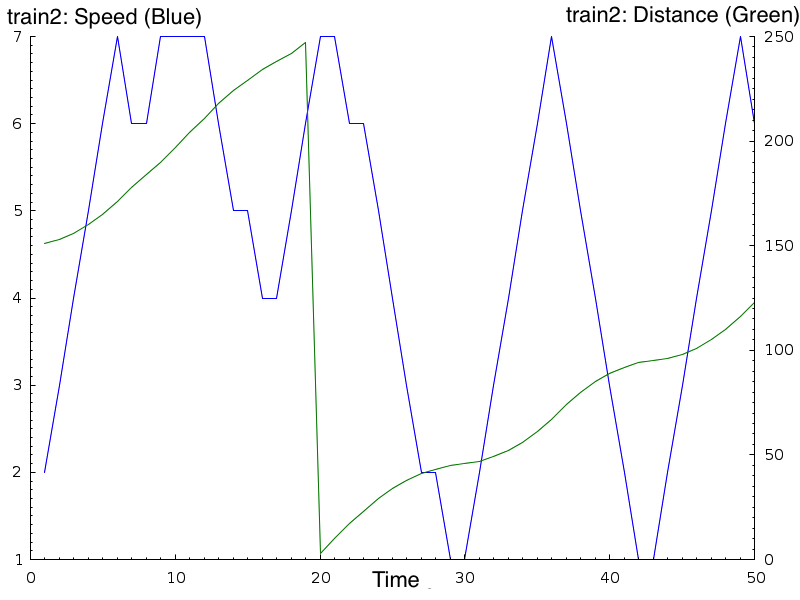
\includegraphics[scale=0.64]{t2graph.png}
\end{center}
\caption{A graph comparing the distance and speed of train2}
\end{figure}

\begin{figure}
\label{t1t2graph}
\begin{center}
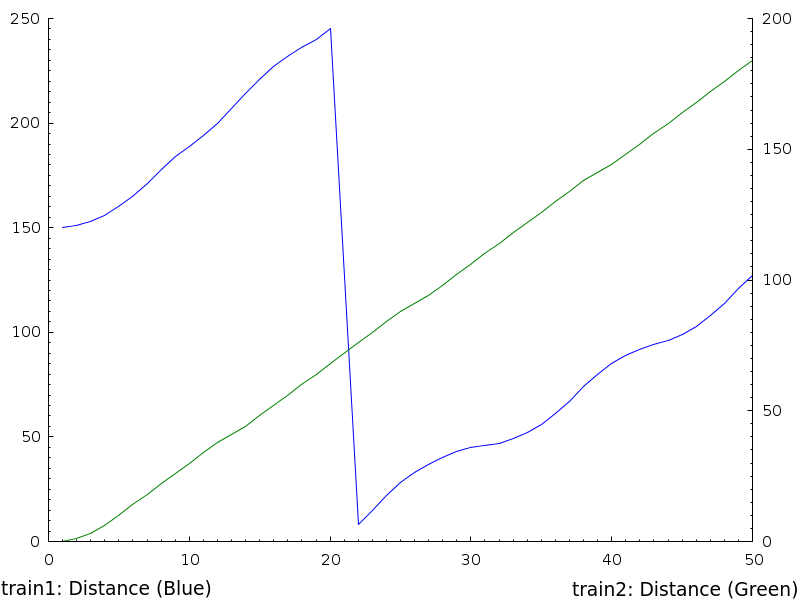
\includegraphics[scale=0.64]{t1t2graph.png}
\end{center}
\caption{A graph comparing the distances of train1 and train2}
\end{figure}

In fig \ref{t1t2} we see that train2 never enters the same track segment as train1.

\section{The Maude Linear Temporal Logic Model Checker}
The Real Time Maude system includes a model checker for linear temporal logic \cite{ES00}.  This is a useful automatic tool which allows for the verification and analysis of real time systems. In addition to the positive verification results in which a safety property holds,  the system produces, in the case of a negative verification result, a counter example trace which shows the. In the following we shall present formal definitions for linear temporal logic and the model checking problem for formulae in this logic.

 

\section{Model Checking the European Rail Traffic Management System}
In the following section we will demonstrate an approach to apply the Real Time Maude LTL model checker to verify the Real Time Maude specification described previously.
Firstly we shall define the property we want to check in the Real Time Maude system. To do this we have to define a satisfaction relation which describes what it means for the property to hold in a state of the system we are checking.  The property we shall consider in this case is that the moment authorities of two trains in system do not overlap. Logical property we define identifies the individual trains using their object identifiers and then computes whether or not an over lap has occurred using a boolean formula.  We shall show that it is possible to verify this property over a time period large enough for all normal behaviours of the system to occur. 

\subsection*{Defining a Satisfaction Relation}
The syntax of the properties for which we are going to check using the LTL model checker are defined separately from the semantics in terms of a satisfaction relation.
We shall now describe how to define the behaviour of the satisfaction relation for a given system and property as a Real Time Maude specification. The satisfaction relation itself is predefined in a specification as an operation which takes a State and a property which is of type Prop and computes a boolean. Maude defines the satisfaction relation $\models$ in the following:
\medskip

\begin{lstlisting}[caption =  The Maude Satisfaction module, label =code:satisfaction ]
  fmod SATISFACTION is  
    protecting BOOL .  
    sorts State Prop .  
    op _|=_ : State Prop -> Bool [frozen] .  
  endfm
\end{lstlisting}
\medskip
The sorts \texttt{State} and \texttt{Prop} are undefined as is the behaviour of $\models$. It is left to the user of the model checker to define the behaviour for their own purposes. The standard way to define predicates which refer to a given object is by matching object identifiers.

We can check that a train is in a specific state as follows:
\begin{lstlisting}[caption = The constant speed property]
ops train-cons : Oid -> Prop [ctor] .
eq {REST < O1 : Train | state : cons >} |= train-cons(O1') 
   = (O1 == O1') . 
\end{lstlisting}
This predicate holds if there is a train in t he configuration with object identifier O1' and a state cons. 

We can check that a train has a certain speed as follows:
\begin{lstlisting}[caption = The speed property]
op train-s : Oid Nat -> Prop [ctor] .
eq {REST < O1 : Train | speed : N1 >} |= train-s(O1',N1') = 
   (N1 == N1') and (O1 == O1') .
\end{lstlisting}

Here the natural number N1 in the train object is matched with N1' in the predicate train-s.
The main movement authority that we want to check is that the movement authorities of two trains does not over lap.
To do this we define a Property nomaoverlap(O1,O2) of type \texttt{Oid Oid -> Prop [ctor]} as follows: 

\begin{lstlisting}
eq {REST < O1 : Train |  dist : D1 , ma : M1 > 
   < O2 : Train |  dist : D2 , ma : M2 >} |= nomaoverlap(O1',O2') = 
   (O1 == O1') and (O2 == O2') and noolap(D1,M1,D2,M2) .
\end{lstlisting}
Here we have matched two object identifiers and natural numbers and called a boolean function \texttt{noolap} on those variables. This definition features an external operation which computes a boolean depending on whether a set of inequalities are satisfied. 

\begin{lstlisting}[caption = The no overlap operation]
eq noolap(D1,M1,D2,M2) = 
   ((D1 < M1) and (M1 < D2) and (D2 < M2)) or 
   ((D2 < M2) and (M2 < D1) and (D1 < M1)) or 
   ((D1 < M1) and (M2 < D1) and (M1 < D2)) or 
   ((D2 < M2) and (M1 < D2) and (M2 < D1) )  .  
\end{lstlisting}

This external operation encodes the 4 possible combines of movement authorities and trains in which the movement authorities do not over lap.  The first case is that train one is behind its movement authority which is behind the second train which itself is behind the movement authority. The second case is the reverse of the first case. In the third and fourth cases  one of the trains is behind its movement authority and the other is towards the end of the track and has its movement authority extended into the initial segment at the beginning of the track.

\subsection{Execution of The LTL Model Checker}
\textbf{Note: do we want to describe and verify other safety conditions here?}
We shall now describe the execution of the LTL model checker in Real Time Maude. This is done using the mc command with some initial state of type system, a satisfaction relation, the LTL formula to be checked and an optional time. The satisfaction relation can be either $\models_u$ for un-timed model checking for which time is not specified or $\models_t$ for which the optional time is specified.

The Real Time Maude LTL model checker is then called using the following command:

\begin{center}
\texttt{(mc initialstate2 |=t [] nomaoverlap(train1,train2) in time <= 30 .)}
\end{center}
The command states that we are applying timed model checking to check that it is globally true that the movement authorities of the trains do not over lap at all moments in time less than or equal to 30. This results in the following output from Real Time Maude which indicates that the property was succesfully verified in 3 minutes and 22 seconds taking the system approximately 140 million rewrites.
\begin{lstlisting}[caption = No overlapping movement authorities model checking result]
rewrites: 138889387 in 179663ms cpu 
(202024ms real) (773054 rewrites/second)

Model check initialstate2 |=t[]nomaoverlap(train1,train2)in 
MODEL-CHECK-ERTMS8 in time <= 30 
with mode deterministic time increase

Result Bool :
  true
\end{lstlisting}

Unfortunately the Real Time Maude LTL model checker can not detect the congruence between difference configurations of control system. Therefore the state space is infinite and it is impossible to do untimed model checking on the above model checking problem. It is however possible to do timed model checking within a reasonable time limit that allows for all behaviours of the system to be verified.

\section{Conclusion}
 We have presented the first attempt at modelling and verifying the combined ERTMS and interlocking system.
\subsection*{Future Work}
There are numerous ways in which our model can be extended. One of the biggest problems facing engineers when developing the ERTMS system is time and how it affects the transition of messages with delays often occurring. This could be easily be modelled following the work \cite{PO07} where delays are modelled in the communications between nodes of a wireless sensor network. Currently our trains have a jerky behaviour in terms of speed, breaking and accelerating in rapid succession there are several other behaviours that trains exhibit in real life that we have not captured in our model. Trains have the ability to coast where the engine in not powering the train but the brakes are not active which is used for several purposes. To save energy coasting and accelerating are often combined to hold the train at max speed. The trains may also coast before breaking when reaching the end of a movement authority.

Currently the track is closed and trains are capable of looping round the track giving it an infinite state space. Opening up the track with an entrance and exit would provide the opportunity to model the hand over part of the protocol where new trains must register with the RBC on entering the track and then de-register upon leaving. This opening of the track would also finitise the state space possibly allowing for un-timed model checking to take place. This example could then be extended by increasing the complexity of the track further and then modelling routes and points. This would allow for the checking of a further safety conditions that states no train has a movement authority over a point in locked in the wrong direction or a moving point.

The RBC has the possibility to pre-emptively grant movement authorities to trains without them requesting it in the case that a train is on a route which contains free sections of track behind a movement authority.  The trains could also request movement authorities before the point at which we reach the braking point.